\documentclass[tikz,border=2pt]{standalone}
\usepackage{amsmath,amssymb}
\usepackage{pgfplots}
\usepgfplotslibrary{groupplots}
\pgfplotsset{compat=1.18}

\begin{document}
% Three joint behaviours: an exact decreasing line (correlation -1), a positive cloud
% (sample correlation 0.74), and Y = X^2 with X symmetric (correlation 0 although Y depends on X).
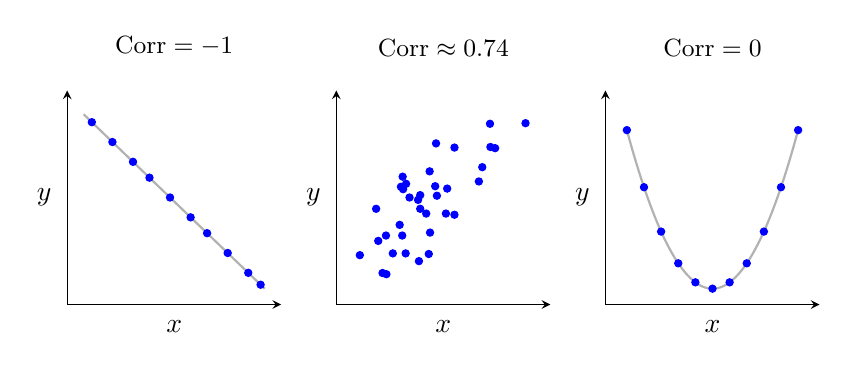
\begin{tikzpicture}
	\begin{groupplot}[
		group style={group size=3 by 1, horizontal sep=7mm},
		width=4.3cm, height=4.3cm, axis lines=left, xtick=\empty, ytick=\empty,
		xlabel={$x$}, ylabel={$y$}, ylabel style={rotate=-90},
		title style={font=\small, yshift=1mm}, clip=false
		]
		\nextgroupplot[title={$\operatorname{Corr}=-1$}, xmin=-0.2, xmax=2.4, ymin=0.2, ymax=5.6]
		\addplot[gray!60, thick, domain=0:2.2] {5-2*x};
		\addplot[only marks, mark=*, mark size=1.3pt, blue] coordinates {(0.1,4.8) (0.35,4.3) (0.6,3.8) (0.8,3.4) (1.05,2.9) (1.3,2.4) (1.5,2.0) (1.75,1.5) (2.0,1.0) (2.15,0.7)};
		\nextgroupplot[title={$\operatorname{Corr}\approx0.74$}, xmin=0.8, xmax=5.8, ymin=0.3, ymax=3.9]
		\addplot[only marks, mark=*, mark size=1.3pt, blue] coordinates {(5.22,3.35) (2.71,2.06) (1.78,1.37) (2.12,1.16) (4.40,2.95) (1.73,1.91) (1.88,0.83) (3.56,1.81) (2.42,1.16) (2.28,1.64) (2.51,2.10) (2.98,2.54) (2.90,1.83) (2.76,1.91) (3.56,2.94) (2.31,2.28) (3.36,1.83) (3.11,2.29) (2.43,2.33) (4.21,2.61) (2.76,2.14) (4.39,3.34) (3.39,2.25) (2.99,1.51) (2.35,2.45) (4.51,2.93) (3.13,3.01) (2.73,1.03) (1.97,0.81) (2.96,1.15) (1.35,1.13) (4.13,2.37) (2.34,1.46) (3.15,2.13) (2.36,2.24) (1.96,1.46)};
		\nextgroupplot[title={$\operatorname{Corr}=0$}, xmin=-1.25, xmax=1.25, ymin=-0.1, ymax=1.25]
		\addplot[gray!60, thick, domain=-1:1, samples=60] {x^2};
		\addplot[only marks, mark=*, mark size=1.3pt, blue] coordinates {(-1.0,1.00) (-0.8,0.64) (-0.6,0.36) (-0.4,0.16) (-0.2,0.04) (0.0,0.00) (0.2,0.04) (0.4,0.16) (0.6,0.36) (0.8,0.64) (1.0,1.00)};
	\end{groupplot}
	
\end{tikzpicture}
\end{document}
